% Created 2019-06-29 sáb 20:44
% Intended LaTeX compiler: pdflatex
\documentclass[xcolor={usenames,svgnames,dvipsnames}]{beamer}
\usepackage[utf8]{inputenc}
\usepackage[T1]{fontenc}
\usepackage{graphicx}
\usepackage{grffile}
\usepackage{longtable}
\usepackage{wrapfig}
\usepackage{rotating}
\usepackage[normalem]{ulem}
\usepackage{amsmath}
\usepackage{textcomp}
\usepackage{amssymb}
\usepackage{capt-of}
\usepackage{hyperref}
\usepackage{color}
\usepackage{listings}
\usepackage{mathpazo}
\usepackage{gensymb}
\usepackage{amsmath}
\usepackage{esdiff}
\usepackage{steinmetz}
\bibliographystyle{plain}
\AtBeginSubsection[]{\begin{frame}[plain]\tableofcontents[currentsubsection,sectionstyle=show/shaded,subsectionstyle=show/shaded/hide]\end{frame}}
\AtBeginSection[]{\begin{frame}[plain]\tableofcontents[currentsection,hideallsubsections]\end{frame}}
\usepackage[emulate=units]{siunitx}
\sisetup{fraction=nice, decimalsymbol=comma, retain-unity-mantissa = false}
\newunit{\wattpeak}{Wp}
\newunit{\watthour}{Wh}
\newunit{\amperehour}{Ah}
\hypersetup{colorlinks=true, linkcolor=Blue, urlcolor=Blue}
\renewcommand{\thefootnote}{\fnsymbol{footnote}}
\beamertemplatenavigationsymbolsempty
\setbeamertemplate{footline}[frame number]
\newcommand{\laplace}[1]{\mathbf{#1}(\mathbf{s})}
\newcommand{\slp}{\mathbf{s}}
\newcommand{\fasor}[1]{\mathbf{#1}(\omega)}
\newcommand{\atan}{\mathrm{atan}}
\setbeamercolor{alerted text}{fg=blue!50!black} \setbeamerfont{alerted text}{series=\bfseries}
\usetheme[hideothersubsections]{Goettingen}
\usecolortheme{rose}
\usefonttheme{serif}
\author{Oscar Perpiñán Lamigueiro}
\date{Diciembre 2018}
\title{Cuadripolos}
\subtitle{Teoría de Circuitos III}
\hypersetup{
 pdfauthor={Oscar Perpiñán Lamigueiro},
 pdftitle={Cuadripolos},
 pdfkeywords={},
 pdfsubject={},
 pdfcreator={Emacs 26.1 (Org mode 9.2)}, 
 pdflang={Spanish}}
\begin{document}

\maketitle

\section{Introducción}
\label{sec:org126df39}

\begin{frame}[label={sec:org4b549c6}]{Cuadripolo}
\begin{center}
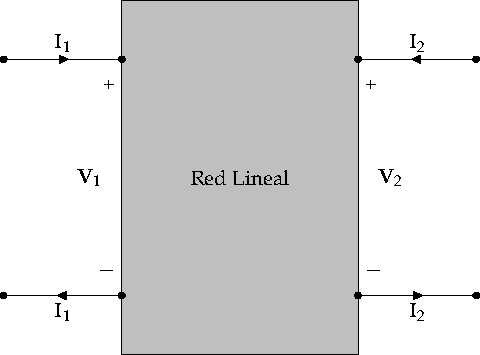
\includegraphics[width=.9\linewidth]{../figs/cuadripolo.pdf}
\end{center}

\begin{center}
\alert{Atención al sentido de las corrientes}
\end{center}
\end{frame}
\begin{frame}[label={sec:org3661f0f}]{Cuadripolos Recíprocos y Simétricos}
\begin{itemize}
\item Un cuadripolo es \alert{recíproco} si, al intercambiar la posición de las excitaciones, la respuesta en el puerto correspondiente no sufre cambios (teorema de reciprocidad).
\item Un cuadripolo lineal (RLC) y \alert{sin fuentes dependientes} es recíproco.
\item Un \alert{cuadripolo recíproco es simétrico} si se puede intercambiar la entrada con la salida (simetría física).
\end{itemize}
\end{frame}
\section{Parámetros de Cuadripolos}
\label{sec:orgb72d75d}
\subsection{Parámetros de Impedancia}
\label{sec:org39850c0}

\begin{frame}[label={sec:org4a5c1ec}]{Definición}
\begin{center}
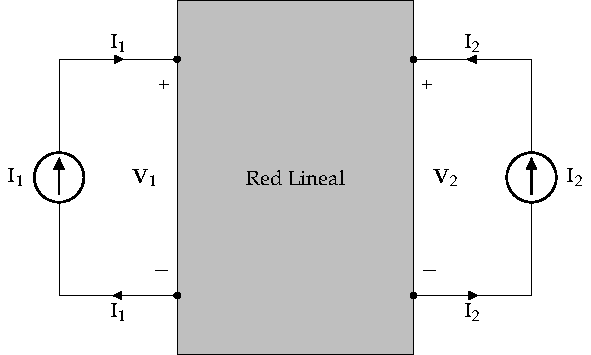
\includegraphics[width=.9\linewidth]{../figs/cuadripolo_fuentes_corriente.pdf}
\end{center}

Mediante teorema de superposición:
\[
\begin{array}{l}
  \mathbf{V}_1 = \mathbf{z}_{11} \mathbf{I}_1 + \mathbf{z}_{12} \mathbf{I}_2\\
  \mathbf{V}_2 = \mathbf{z}_{21} \mathbf{I}_1 + \mathbf{z}_{22} \mathbf{I}_2\\
\end{array}
\]

Las variables independientes (\emph{generadores}) son \(\mathbf{I}_1\) e \(\mathbf{I}_2\).
\end{frame}

\begin{frame}[label={sec:org811a092}]{Expresión Matricial}
\begin{center}
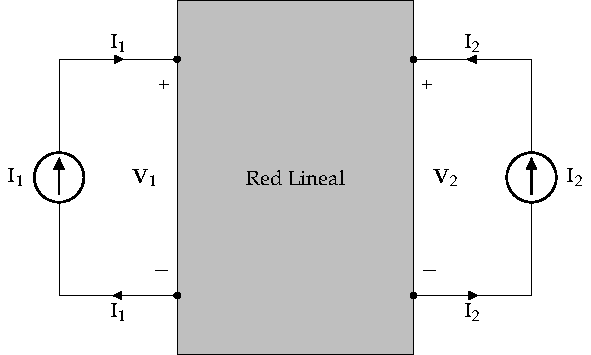
\includegraphics[width=.9\linewidth]{../figs/cuadripolo_fuentes_corriente.pdf}
\end{center}

\[
  \left[
    \begin{array}{c}
      \mathbf{V}_1\\
      \mathbf{V}_2
    \end{array}
  \right] =
  \left[
    \begin{array}{cc}
      \mathbf{z}_{11} & \mathbf{z}_{12}\\
      \mathbf{z}_{21} & \mathbf{z}_{22}
    \end{array}
  \right] \cdot
  \left[
    \begin{array}{c}
      \mathbf{I}_1\\
      \mathbf{I}_2
    \end{array}
  \right]
\]
\end{frame}

\begin{frame}[label={sec:orgba38928}]{Circuito Equivalente}
\begin{center}
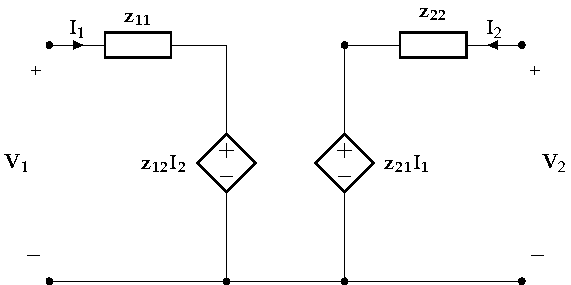
\includegraphics[width=.9\linewidth]{../figs/circuitoEquivalenteZ.pdf}
\end{center}

\[
\begin{array}{l}
  \mathbf{V}_1 = \mathbf{z}_{11} \mathbf{I}_1 + \mathbf{z}_{12} \mathbf{I}_2\\
  \mathbf{V}_2 = \mathbf{z}_{21} \mathbf{I}_1 + \mathbf{z}_{22} \mathbf{I}_2\\
\end{array}
\]
\end{frame}

\begin{frame}[label={sec:org27ce7f7}]{Cálculo de parámetros}
\begin{block}{Salida en abierto}
\begin{columns}
\begin{column}{0.3\columnwidth}
\renewcommand{\arraystretch}{2}
\[
  \begin{array}{c}
    \mathbf{z}_{11} = \left.\frac{\mathbf{V}_1}{\mathbf{I}_1}\right\rvert_{\mathbf{I}_2 = 0} \\
    \mathbf{z}_{21} = \left.\frac{\mathbf{V}_2}{\mathbf{I}_1}\right\rvert_{\mathbf{I}_2 = 0}
  \end{array}
\]
\end{column}

\begin{column}{0.7\columnwidth}
\begin{center}
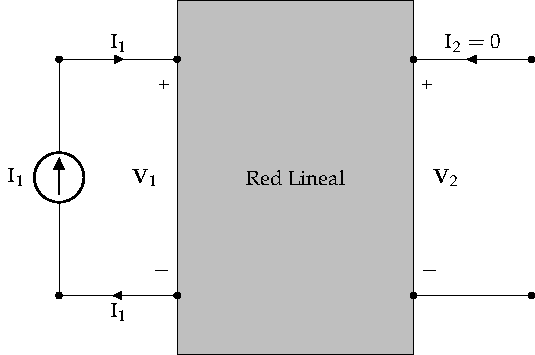
\includegraphics[width=.9\linewidth]{../figs/parametrosZ_entrada.pdf}
\end{center}
\end{column}
\end{columns}
\end{block}

\[
  \left[
    \begin{array}{c}
      \mathbf{V}_1\\
      \mathbf{V}_2
    \end{array}
  \right] =
  \left[
    \begin{array}{cc}
      \color{blue}{\mathbf{z}_{11}} & \mathbf{z}_{12}\\
      \color{blue}{\mathbf{z}_{21}} & \mathbf{z}_{22}
    \end{array}
  \right] \cdot
  \left[
    \begin{array}{c}
      \color{blue}{\mathbf{I}_1}\\
      \mathbf{I}_2
    \end{array}
  \right]
\]
\end{frame}

\begin{frame}[label={sec:orgb3ef06f}]{Cálculo de parámetros}
\begin{block}{Entrada en abierto}
\begin{columns}
\begin{column}{0.75\columnwidth}
\begin{center}
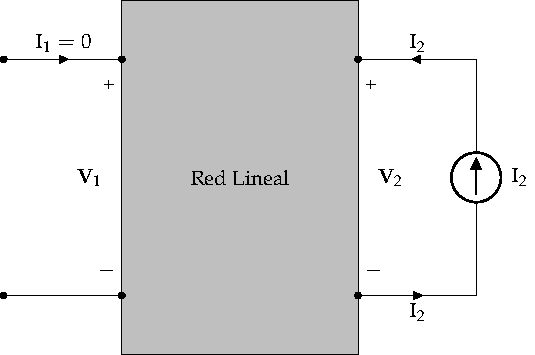
\includegraphics[width=.9\linewidth]{../figs/parametrosZ_salida.pdf}
\end{center}
\end{column}

\begin{column}{0.25\columnwidth}
\renewcommand{\arraystretch}{2}
\[
  \begin{array}{c}
    \mathbf{z}_{12} = \left.\frac{\mathbf{V}_1}{\mathbf{I}_2}\right\rvert_{\mathbf{I}_1 = 0}\\
    \mathbf{z}_{22} = \left.\frac{\mathbf{V}_2}{\mathbf{I}_2}\right\rvert_{\mathbf{I}_1 = 0}
  \end{array}
\]
\end{column}
\end{columns}
\end{block}

\[
  \left[
    \begin{array}{c}
      \mathbf{V}_1\\
      \mathbf{V}_2
    \end{array}
  \right] =
  \left[
    \begin{array}{cc}
      \mathbf{z}_{11} & \color{blue}{\mathbf{z}_{12}}\\
      \mathbf{z}_{21} & \color{blue}{\mathbf{z}_{22}}
    \end{array}
  \right] \cdot
  \left[
    \begin{array}{c}
      \mathbf{I}_1\\
      \color{blue}{\mathbf{I}_2}
    \end{array}
  \right]
\]
\end{frame}

\begin{frame}[label={sec:orgc499e8a}]{Reciprocidad}
\[
\left.\mathbf{V_1}\right\rvert_{
  \begin{array}{l}
\mathbf{I_1} = 0\\ \mathbf{I_2} = \mathbf{I_x}
  \end{array}
} =% 
\left.\mathbf{V_2}\right\rvert_{
  \begin{array}{l}
\mathbf{I_2} = 0\\ \mathbf{I_1} = \mathbf{I_x}
  \end{array}
}
\]

\begin{columns}
\begin{column}{0.5\columnwidth}
\begin{center}
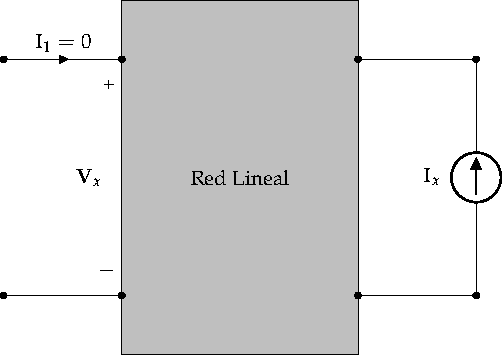
\includegraphics[width=.9\linewidth]{../figs/reciprocidadZ_entrada.pdf}
\end{center}
\end{column}
\begin{column}{0.5\columnwidth}
\begin{center}
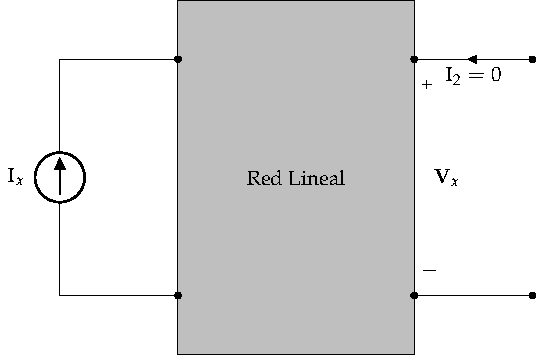
\includegraphics[width=.9\linewidth]{../figs/reciprocidadZ_salida.pdf}
\end{center}
\end{column}
\end{columns}
\end{frame}
\begin{frame}[label={sec:org76dca4e}]{Relación entre parámetros}
Las impedancias de transferencia son idénticas
\[
  \left.
    \begin{array}{l}
      \mathbf{V}_x = \mathbf{z}_{11} 0  + \mathbf{z}_{12} \mathbf{I}_x\\
      \mathbf{V}_x = \mathbf{z}_{21} \mathbf{I}_x + \mathbf{z}_{22} 0\\
    \end{array} \right\} \rightarrow \boxed{\mathbf{z_{12}} = \mathbf{z_{21}}}
\]

\begin{columns}
\begin{column}{0.5\columnwidth}
\begin{center}
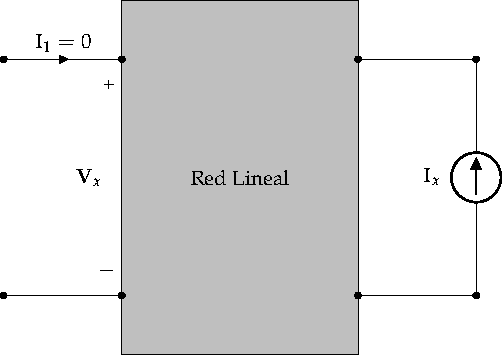
\includegraphics[width=.9\linewidth]{../figs/reciprocidadZ_entrada.pdf}
\end{center}
\end{column}
\begin{column}{0.5\columnwidth}
\begin{center}
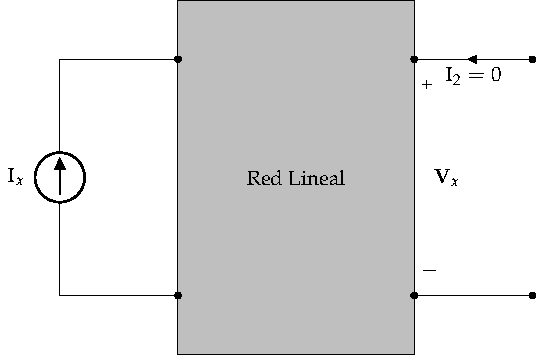
\includegraphics[width=.9\linewidth]{../figs/reciprocidadZ_salida.pdf}
\end{center}
\end{column}
\end{columns}
\end{frame}

\begin{frame}[label={sec:orgb419fb2}]{Circuito Equivalente en T}
\[
\boxed{\mathbf{z_{12}} = \mathbf{z_{21}}}
\rightarrow
\left[
    \begin{array}{c}
      \mathbf{V}_1\\
      \mathbf{V}_2
    \end{array}
  \right] =
  \left[
    \begin{array}{cc}
      \mathbf{z}_{11} & \color{red}{\mathbf{z}_{12}}\\
      \color{red}{\mathbf{z}_{12}} & \mathbf{z}_{22}
    \end{array}
  \right] \cdot
  \left[
    \begin{array}{c}
      \mathbf{I}_1\\
      \mathbf{I}_2
    \end{array}
  \right]
\]

\begin{block}{Ejercicio}
Demostrar que un cuadripolo recíproco es equivalente al circuito en T de la figura.

\begin{center}
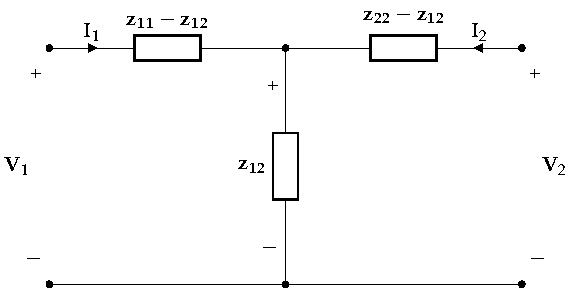
\includegraphics[width=.9\linewidth]{../figs/circuitoEquivalenteZReciproco.pdf}
\end{center}
\end{block}
\end{frame}

\begin{frame}[label={sec:orgf0e805c}]{Cuadripolo Simétrico}
\begin{center}
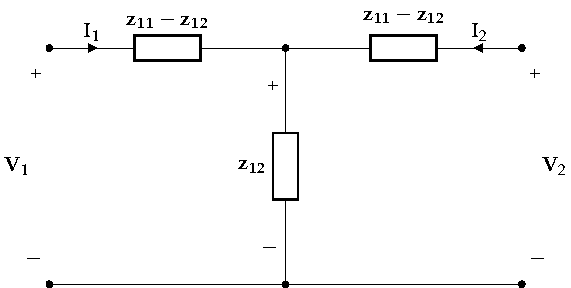
\includegraphics[width=.9\linewidth]{../figs/circuitoEquivalenteZSimetrico.pdf}
\end{center}

\[
\boxed{\mathbf{z_{11}} = \mathbf{z_{22}}}
\rightarrow
\left[
    \begin{array}{c}
      \mathbf{V}_1\\
      \mathbf{V}_2
    \end{array}
  \right] =
  \left[
    \begin{array}{cc}
      \color{blue}{\mathbf{z}_{11}} & \color{red}{\mathbf{z}_{12}}\\
      \color{red}{\mathbf{z}_{12}} & \color{blue}{\mathbf{z}_{11}}
    \end{array}
  \right] \cdot
  \left[
    \begin{array}{c}
      \mathbf{I}_1\\
      \mathbf{I}_2
    \end{array}
  \right]
\]
\end{frame}


\begin{frame}[label={sec:orgaa2b649}]{No siempre hay parámetros Z}
¿Cuáles son los parámetros Z \ldots{} 

\begin{itemize}
\item de un transformador ideal?
\item de una impedancia serie?
\end{itemize}
\end{frame}

\subsection{Parámetros de Admitancia}
\label{sec:orge1a5d97}
\begin{frame}[label={sec:org9a38a95}]{Definición}
\begin{center}
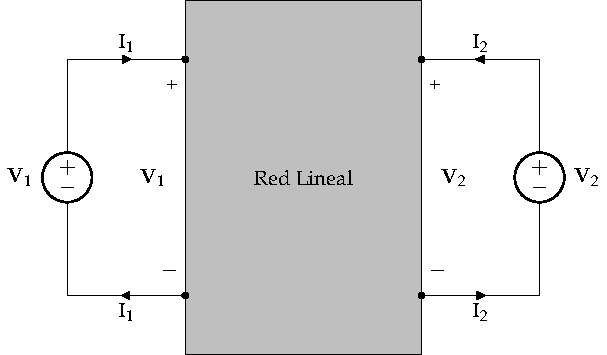
\includegraphics[width=.9\linewidth]{../figs/cuadripolo_fuentes_tension.pdf}
\end{center}

Mediante teorema de superposición:
\[
\begin{array}{l}
  \mathbf{I}_1 = \mathbf{y}_{11} \mathbf{V}_1 + \mathbf{y}_{12} \mathbf{V}_2\\
  \mathbf{I}_2 = \mathbf{y}_{21} \mathbf{V}_1 + \mathbf{y}_{22} \mathbf{V}_2\\
\end{array}
\]

Las variables independientes (\emph{generadores}) son \(\mathbf{V}_1\) e \(\mathbf{V}_2\).
\end{frame}

\begin{frame}[label={sec:org80de73d}]{Expresión Matricial}
\begin{center}
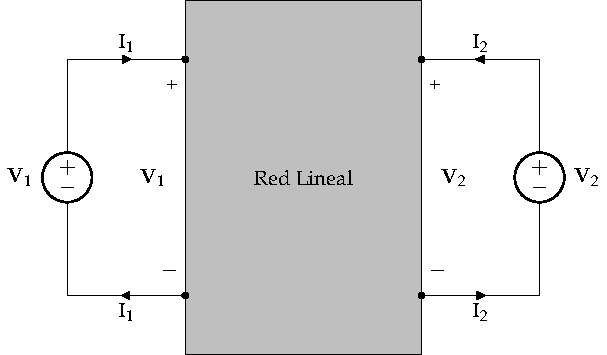
\includegraphics[width=.9\linewidth]{../figs/cuadripolo_fuentes_tension.pdf}
\end{center}

\[
  \left[
    \begin{array}{c}
      \mathbf{I}_1\\
      \mathbf{I}_2
    \end{array}
  \right] =
  \left[
    \begin{array}{cc}
      \mathbf{y}_{11} & \mathbf{y}_{12}\\
      \mathbf{y}_{21} & \mathbf{y}_{22}
    \end{array}
  \right] \cdot
  \left[
    \begin{array}{c}
      \mathbf{V}_1\\
      \mathbf{V}_2
    \end{array}
  \right]
\]
\end{frame}

\begin{frame}[label={sec:org729b0c4}]{Circuito Equivalente}
\begin{center}
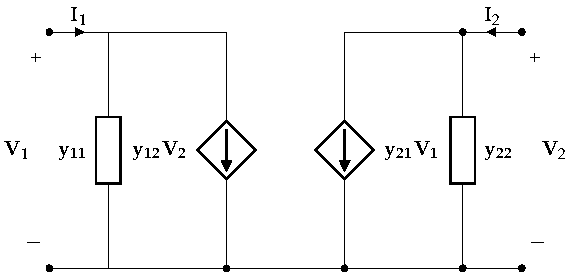
\includegraphics[width=.9\linewidth]{../figs/circuitoEquivalenteY.pdf}
\end{center}

\[
\begin{array}{l}
  \mathbf{I}_1 = \mathbf{y}_{11} \mathbf{V}_1 + \mathbf{y}_{12} \mathbf{V}_2\\
  \mathbf{I}_2 = \mathbf{y}_{21} \mathbf{V}_1 + \mathbf{y}_{22} \mathbf{V}_2\\
\end{array}
\]
\end{frame}


\begin{frame}[label={sec:org662b7f0}]{Cálculo de parámetros}
\begin{block}{Salida en cortocircuito}
\begin{columns}
\begin{column}{0.3\columnwidth}
\renewcommand{\arraystretch}{2}
\[
  \begin{array}{c}
    \mathbf{y}_{11} = \left.\frac{\mathbf{I}_1}{\mathbf{V}_1}\right\rvert_{\mathbf{V}_2 = 0} \\
    \mathbf{y}_{21} = \left.\frac{\mathbf{I}_2}{\mathbf{V}_1}\right\rvert_{\mathbf{V}_2 = 0}
  \end{array}
\]
\end{column}

\begin{column}{0.7\columnwidth}
\begin{center}
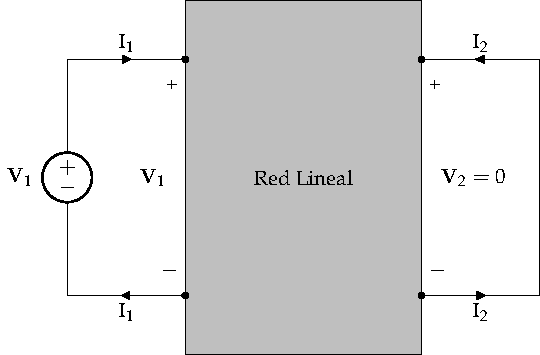
\includegraphics[width=.9\linewidth]{../figs/parametrosY_entrada.pdf}
\end{center}
\end{column}
\end{columns}
\end{block}

\[
  \left[
    \begin{array}{c}
      \mathbf{I}_1\\
      \mathbf{I}_2
    \end{array}
  \right] =
  \left[
    \begin{array}{cc}
      \color{blue}{\mathbf{y}_{11}} & \mathbf{y}_{12}\\
      \color{blue}{\mathbf{y}_{21}} & \mathbf{y}_{22}
    \end{array}
  \right] \cdot
  \left[
    \begin{array}{c}
      \color{blue}{\mathbf{V}_1}\\
      \mathbf{V}_2
    \end{array}
  \right]
\]
\end{frame}


\begin{frame}[label={sec:org396ce1b}]{Cálculo de parámetros}
\begin{block}{Entrada en cortocircuito}
\begin{columns}
\begin{column}{0.7\columnwidth}
\begin{center}
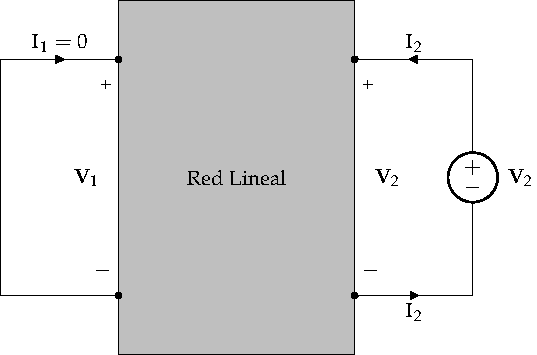
\includegraphics[width=.9\linewidth]{../figs/parametrosY_salida.pdf}
\end{center}
\end{column}

\begin{column}{0.3\columnwidth}
\renewcommand{\arraystretch}{2}
\[
  \begin{array}{c}
    \mathbf{y}_{12} = \left.\frac{\mathbf{I}_1}{\mathbf{V}_2}\right\rvert_{\mathbf{V}_1 = 0}\\
    \mathbf{y}_{22} = \left.\frac{\mathbf{I}_2}{\mathbf{V}_2}\right\rvert_{\mathbf{V}_1 = 0}
  \end{array}
\]
\end{column}
\end{columns}
\end{block}

\[
  \left[
    \begin{array}{c}
      \mathbf{I}_1\\
      \mathbf{I}_2
    \end{array}
  \right] =
  \left[
    \begin{array}{cc}
      \mathbf{y}_{11} & \color{blue}{\mathbf{y}_{12}}\\
      \mathbf{y}_{21} & \color{blue}{\mathbf{y}_{22}}
    \end{array}
  \right] \cdot
  \left[
    \begin{array}{c}
      \mathbf{V}_1\\
      \color{blue}{\mathbf{V}_2}
    \end{array}
  \right]
\]
\end{frame}

\begin{frame}[label={sec:org784a1c5}]{Reciprocidad}
\[
\mathbf{I_1}\rvert_{
  \begin{array}{l}
\mathbf{V_1} = 0 \\ \mathbf{V_2} = \mathbf{V_x}
  \end{array}
} =% 
\mathbf{I_2}\rvert_{
  \begin{array}{l}
\mathbf{V_2} = 0 \\ \mathbf{V_1} = \mathbf{V_x}
  \end{array}
}
\]

\begin{columns}
\begin{column}{0.5\columnwidth}
\begin{center}
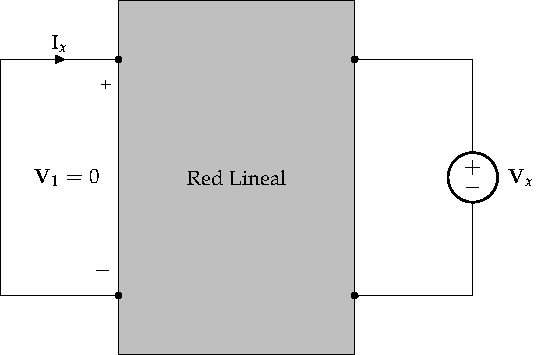
\includegraphics[width=.9\linewidth]{../figs/reciprocidadY_entrada.pdf}
\end{center}
\end{column}
\begin{column}{0.5\columnwidth}
\begin{center}
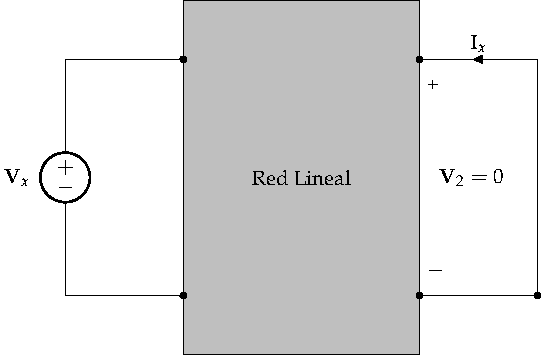
\includegraphics[width=.9\linewidth]{../figs/reciprocidadY_salida.pdf}
\end{center}
\end{column}
\end{columns}
\end{frame}
\begin{frame}[label={sec:org3b98896}]{Relación entre parámetros}
Las admitancias de transferencia son idénticas
\[
  \left.
    \begin{array}{l}
      \mathbf{I}_x = \mathbf{y}_{11} 0  + \mathbf{y}_{12} \mathbf{V}_x\\
      \mathbf{I}_x = \mathbf{y}_{21} \mathbf{V}_x + \mathbf{y}_{22} 0\\
    \end{array} \right\} \rightarrow \boxed{\mathbf{y_{12}} = \mathbf{y_{21}}}
\]

\begin{columns}
\begin{column}{0.5\columnwidth}
\begin{center}
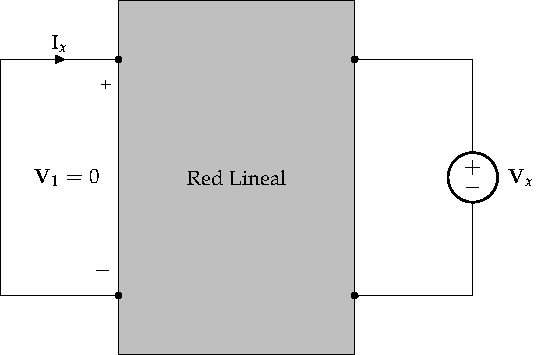
\includegraphics[width=.9\linewidth]{../figs/reciprocidadY_entrada.pdf}
\end{center}
\end{column}
\begin{column}{0.5\columnwidth}
\begin{center}
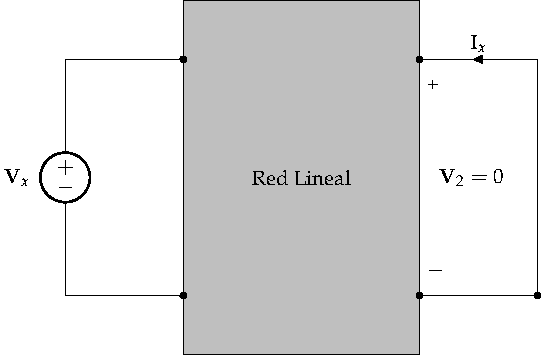
\includegraphics[width=.9\linewidth]{../figs/reciprocidadY_salida.pdf}
\end{center}
\end{column}
\end{columns}
\end{frame}
\begin{frame}[label={sec:orga729f4c}]{Circuito Equivalente en \(\pi\)}
\[
\boxed{\mathbf{y_{12}} = \mathbf{y_{21}}}
\rightarrow
\left[
    \begin{array}{c}
      \mathbf{I}_1\\
      \mathbf{I}_2
    \end{array}
  \right] =
  \left[
    \begin{array}{cc}
      \mathbf{y}_{11} & \color{red}{\mathbf{y}_{12}}\\
      \color{red}{\mathbf{y}_{12}} & \mathbf{y}_{22}
    \end{array}
  \right] \cdot
  \left[
    \begin{array}{c}
      \mathbf{V}_1\\
      \mathbf{V}_2
    \end{array}
  \right]
\]

\begin{block}{Ejercicio}
Demostrar que un cuadripolo recíproco es equivalente al circuito en \(\pi\) de la figura.

\begin{center}
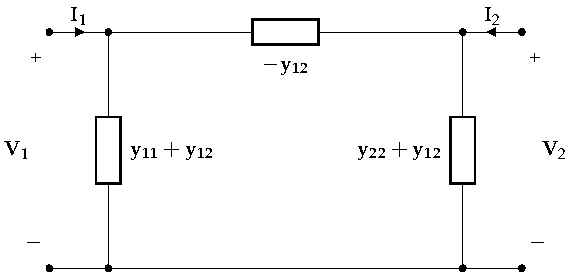
\includegraphics[width=.9\linewidth]{../figs/circuitoEquivalenteYReciproco.pdf}
\end{center}
\end{block}
\end{frame}

\begin{frame}[label={sec:org3640ae1}]{Cuadripolo Simétrico}
\begin{center}
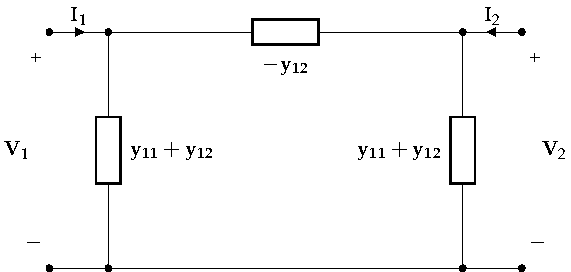
\includegraphics[width=.9\linewidth]{../figs/circuitoEquivalenteYSimetrico.pdf}
\end{center}


\[
\boxed{\mathbf{y_{11}} = \mathbf{y_{22}}}
\rightarrow
\left[
    \begin{array}{c}
      \mathbf{I}_1\\
      \mathbf{I}_2
    \end{array}
  \right] =
  \left[
    \begin{array}{cc}
      \color{blue}{\mathbf{y}_{11}} & \color{red}{\mathbf{y}_{12}}\\
      \color{red}{\mathbf{y}_{12}} & \color{blue}{\mathbf{y}_{11}}
    \end{array}
  \right] \cdot
  \left[
    \begin{array}{c}
      \mathbf{V}_1\\
      \mathbf{V}_2
    \end{array}
  \right]
\]
\end{frame}


\begin{frame}[label={sec:org96f87e5}]{No siempre hay parámetros Y}
¿Cuáles son los parámetros Y \ldots{} 

\begin{itemize}
\item de un transformador ideal?
\item de una impedancia paralelo?
\end{itemize}
\end{frame}

\subsection{Parámetros Híbridos}
\label{sec:org0b8f95a}
\begin{frame}[label={sec:orgb78e277}]{Definición}
\begin{center}
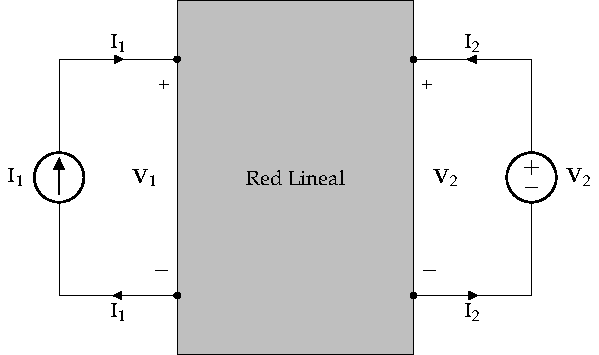
\includegraphics[width=.9\linewidth]{../figs/cuadripolo_hibrido.pdf}
\end{center}

Mediante teorema de superposición:
\[
\begin{array}{l}
  \mathbf{V}_1 = \mathbf{h}_{11} \mathbf{I}_1 + \mathbf{h}_{12} \mathbf{V}_2\\
  \mathbf{I}_2 = \mathbf{h}_{21} \mathbf{I}_1 + \mathbf{h}_{22} \mathbf{V}_2\\
\end{array}
\]

Las variables independientes (\emph{generadores}) son \(\mathbf{I}_1\) e \(\mathbf{V}_2\).
\end{frame}


\begin{frame}[label={sec:org896d140}]{Expresión Matricial}
\begin{center}
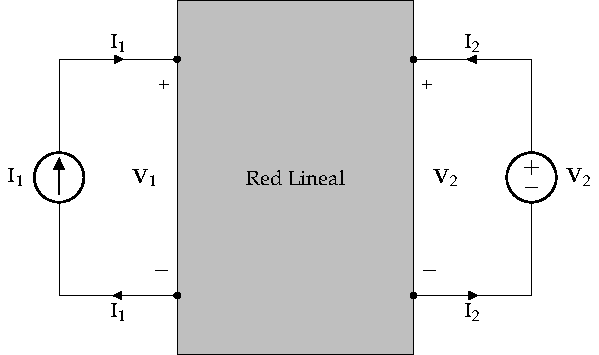
\includegraphics[width=.9\linewidth]{../figs/cuadripolo_hibrido.pdf}
\end{center}

\[
  \left[
    \begin{array}{c}
      \mathbf{V}_1\\
      \mathbf{I}_2
    \end{array}
  \right] =
  \left[
    \begin{array}{cc}
      \mathbf{h}_{11} & \mathbf{h}_{12}\\
      \mathbf{h}_{21} & \mathbf{h}_{22}
    \end{array}
  \right] \cdot
  \left[
    \begin{array}{c}
      \mathbf{I}_1\\
      \mathbf{V}_2
    \end{array}
  \right]
\]
\end{frame}

\begin{frame}[label={sec:orgad86f5e}]{Circuito Equivalente}
\begin{center}
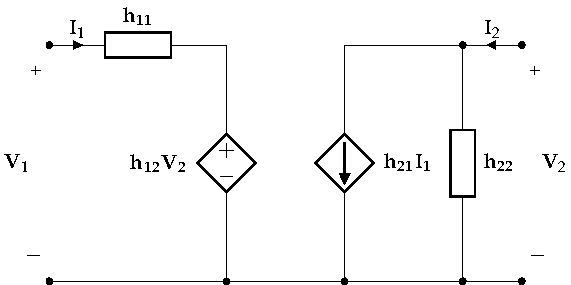
\includegraphics[width=.9\linewidth]{../figs/circuitoEquivalenteH.pdf}
\end{center}

\[
\begin{array}{l}
  \mathbf{V}_1 = \mathbf{h}_{11} \mathbf{I}_1 + \mathbf{h}_{12} \mathbf{V}_2\\
  \mathbf{I}_2 = \mathbf{h}_{21} \mathbf{I}_1 + \mathbf{h}_{22} \mathbf{V}_2\\
\end{array}
\]
\end{frame}

\begin{frame}[label={sec:org4e0aede}]{Cálculo de parámetros}
\begin{block}{Salida en cortocircuito}
\begin{columns}
\begin{column}{0.3\columnwidth}
\renewcommand{\arraystretch}{2}
\[
  \begin{array}{c}
    \mathbf{h}_{11} = \left.\frac{\mathbf{V}_1}{\mathbf{I}_1}\right\rvert_{\mathbf{V}_2 = 0} \\
    \mathbf{h}_{21} = \left.\frac{\mathbf{I}_2}{\mathbf{I}_1}\right\rvert_{\mathbf{V}_2 = 0}
  \end{array}
\]
\end{column}

\begin{column}{0.7\columnwidth}
\begin{center}
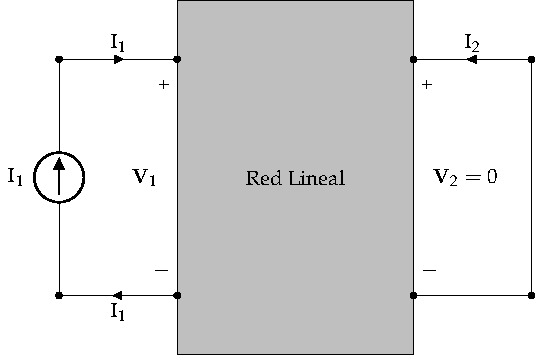
\includegraphics[width=.9\linewidth]{../figs/parametrosH_entrada.pdf}
\end{center}
\end{column}
\end{columns}
\end{block}

\[
  \left[
    \begin{array}{c}
      \mathbf{V}_1\\
      \mathbf{I}_2
    \end{array}
  \right] =
  \left[
    \begin{array}{cc}
      \color{blue}{\mathbf{h}_{11}} & \mathbf{h}_{12}\\
      \color{blue}{\mathbf{h}_{21}} & \mathbf{h}_{22}
    \end{array}
  \right] \cdot
  \left[
    \begin{array}{c}
      \color{blue}{\mathbf{I}_1}\\
      \mathbf{V}_2
    \end{array}
  \right]
\]
\end{frame}

\begin{frame}[label={sec:org48960b8}]{Cálculo de parámetros}
\begin{block}{Entrada en abierto}
\begin{columns}
\begin{column}{0.75\columnwidth}
\begin{center}
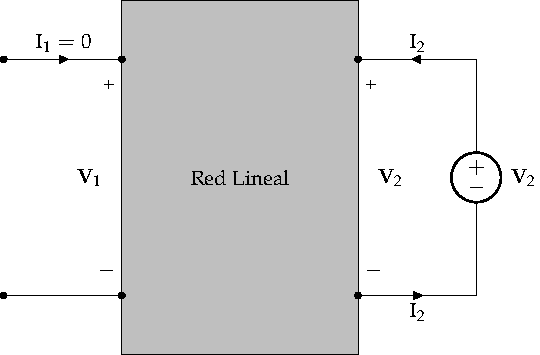
\includegraphics[width=.9\linewidth]{../figs/parametrosH_salida.pdf}
\end{center}
\end{column}

\begin{column}{0.25\columnwidth}
\renewcommand{\arraystretch}{2}
\[
  \begin{array}{c}
    \mathbf{h}_{12} = \left.\frac{\mathbf{V}_1}{\mathbf{V}_2}\right\rvert_{\mathbf{I}_1 = 0}\\
    \mathbf{h}_{22} = \left.\frac{\mathbf{I}_2}{\mathbf{V}_2}\right\rvert_{\mathbf{I}_1 = 0}
  \end{array}
\]
\end{column}
\end{columns}
\end{block}

\[
  \left[
    \begin{array}{c}
      \mathbf{V}_1\\
      \mathbf{I}_2
    \end{array}
  \right] =
  \left[
    \begin{array}{cc}
      \mathbf{h}_{11} & \color{blue}{\mathbf{h}_{12}}\\
      \mathbf{h}_{21} & \color{blue}{\mathbf{h}_{22}}
    \end{array}
  \right] \cdot
  \left[
    \begin{array}{c}
      \mathbf{I}_1\\
      \color{blue}{\mathbf{V}_2}
    \end{array}
  \right]
\]
\end{frame}


\subsection{Parámetros Híbridos Inversos}
\label{sec:orga6c4eb4}

\begin{frame}[label={sec:org912f77e}]{Definición}
\begin{center}
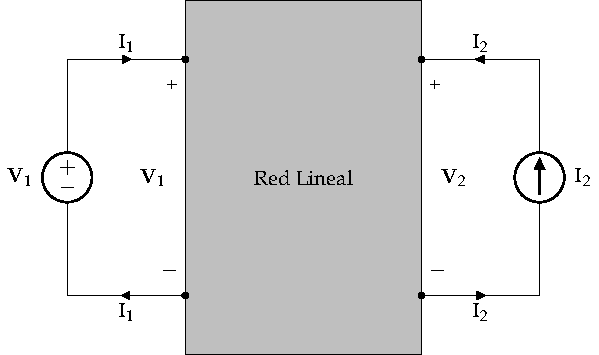
\includegraphics[width=.9\linewidth]{../figs/cuadripolo_hibrido_inverso.pdf}
\end{center}

Mediante teorema de superposición:
\[
\begin{array}{l}
  \mathbf{I}_1 = \mathbf{g}_{11} \mathbf{V}_1 + \mathbf{g}_{12} \mathbf{I}_2\\
  \mathbf{V}_2 = \mathbf{g}_{21} \mathbf{V}_1 + \mathbf{g}_{22} \mathbf{I}_2\\
\end{array}
\]

Las variables independientes (\emph{generadores}) son \(\mathbf{V}_1\) e \(\mathbf{I}_2\).
\end{frame}

\begin{frame}[label={sec:org2dc4c8d}]{Expresión Matricial}
\begin{center}
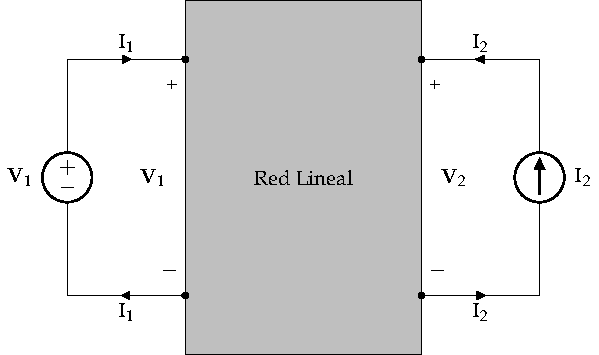
\includegraphics[width=.9\linewidth]{../figs/cuadripolo_hibrido_inverso.pdf}
\end{center}

\[
  \left[
    \begin{array}{c}
      \mathbf{I}_1\\
      \mathbf{V}_2
    \end{array}
  \right] =
  \left[
    \begin{array}{cc}
      \mathbf{g}_{11} & \mathbf{g}_{12}\\
      \mathbf{g}_{21} & \mathbf{g}_{22}
    \end{array}
  \right] \cdot
  \left[
    \begin{array}{c}
      \mathbf{V}_1\\
      \mathbf{I}_2
    \end{array}
  \right]
\]
\end{frame}

\begin{frame}[label={sec:org88c012b}]{Circuito Equivalente}
\begin{center}
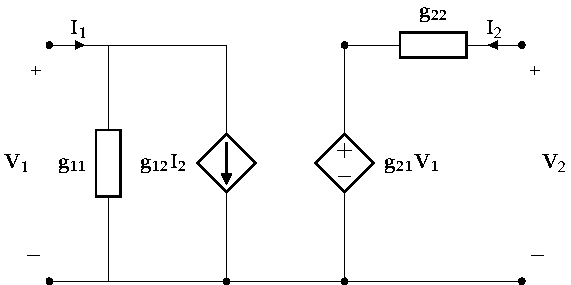
\includegraphics[width=.9\linewidth]{../figs/circuitoEquivalenteG.pdf}
\end{center}

\[
\begin{array}{l}
  \mathbf{I}_1 = \mathbf{g}_{11} \mathbf{V}_1 + \mathbf{g}_{12} \mathbf{I}_2\\
  \mathbf{V}_2 = \mathbf{g}_{21} \mathbf{V}_1 + \mathbf{g}_{22} \mathbf{I}_2\\
\end{array}
\]
\end{frame}

\begin{frame}[label={sec:org8915c5a}]{Cálculo de parámetros}
\begin{block}{Salida en abierto}
\begin{columns}
\begin{column}{0.3\columnwidth}
\renewcommand{\arraystretch}{2}
\[
  \begin{array}{c}
    \mathbf{g}_{11} = \left.\frac{\mathbf{I}_1}{\mathbf{V}_1}\right\rvert_{\mathbf{I}_2 = 0} \\
    \mathbf{g}_{21} = \left.\frac{\mathbf{V}_2}{\mathbf{V}_1}\right\rvert_{\mathbf{I}_2 = 0}
  \end{array}
\]
\end{column}

\begin{column}{0.7\columnwidth}
\begin{center}
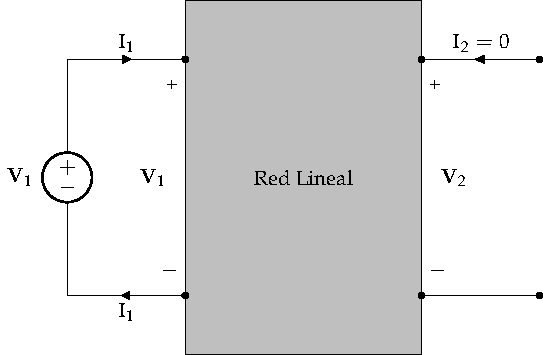
\includegraphics[width=.9\linewidth]{../figs/parametrosG_entrada.pdf}
\end{center}
\end{column}
\end{columns}
\end{block}

\[
  \left[
    \begin{array}{c}
      \mathbf{I}_1\\
      \mathbf{V}_2
    \end{array}
  \right] =
  \left[
    \begin{array}{cc}
      \color{blue}{\mathbf{g}_{11}} & \mathbf{g}_{12}\\
      \color{blue}{\mathbf{g}_{21}} & \mathbf{g}_{22}
    \end{array}
  \right] \cdot
  \left[
    \begin{array}{c}
      \color{blue}{\mathbf{V}_1}\\
      \mathbf{I}_2
    \end{array}
  \right]
\]
\end{frame}

\begin{frame}[label={sec:org2fb7037}]{Cálculo de parámetros}
\begin{block}{Entrada en cortocircuito}
\begin{columns}
\begin{column}{0.7\columnwidth}
\begin{center}
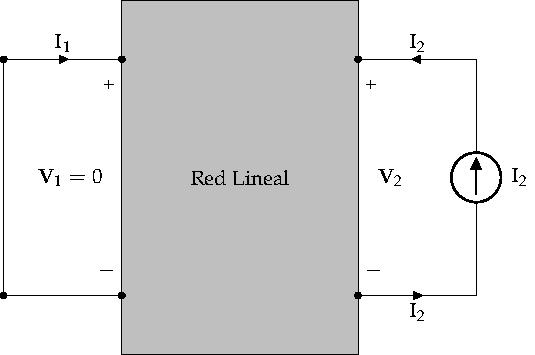
\includegraphics[width=.9\linewidth]{../figs/parametrosG_salida.pdf}
\end{center}
\end{column}

\begin{column}{0.3\columnwidth}
\renewcommand{\arraystretch}{2}
\[
  \begin{array}{c}
    \mathbf{g}_{12} = \left.\frac{\mathbf{I}_1}{\mathbf{I}_2}\right\rvert_{\mathbf{V}_1 = 0}\\
    \mathbf{g}_{22} = \left.\frac{\mathbf{V}_2}{\mathbf{I}_2}\right\rvert_{\mathbf{V}_1 = 0}
  \end{array}
\]
\end{column}
\end{columns}
\end{block}

\[
  \left[
    \begin{array}{c}
      \mathbf{I}_1\\
      \mathbf{V}_2
    \end{array}
  \right] =
  \left[
    \begin{array}{cc}
      \mathbf{g}_{11} & \color{blue}{\mathbf{g}_{12}}\\
      \mathbf{g}_{21} & \color{blue}{\mathbf{g}_{22}}
    \end{array}
  \right] \cdot
  \left[
    \begin{array}{c}
      \mathbf{V}_1\\
      \color{blue}{\mathbf{I}_2}
    \end{array}
  \right]
\]
\end{frame}


\subsection{Parámetros de Transmisión}
\label{sec:org63be55e}

\begin{frame}[label={sec:org2e13f65}]{Definición}
\begin{center}
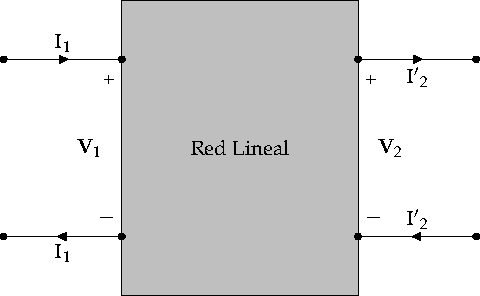
\includegraphics[width=.9\linewidth]{../figs/cuadripolo_transmision.pdf}
\end{center}

\[
\begin{array}{l}
  \mathbf{V}_1 = \mathbf{A} \mathbf{V}_2 + \mathbf{B}\mathbf{I'}_2\\
  \mathbf{I}_1 = \mathbf{C} \mathbf{V}_2 + \mathbf{D} \mathbf{I'}_2\\
\end{array}
\]

\begin{center}
\alert{Atención} al sentido de la corriente \(\mathbf{I'}_2\). (\(\mathbf{I'}_2 = - \mathbf{I}_2\)).
\end{center}
\end{frame}

\begin{frame}[label={sec:orga599d2d}]{Expresión Matricial}
\begin{center}
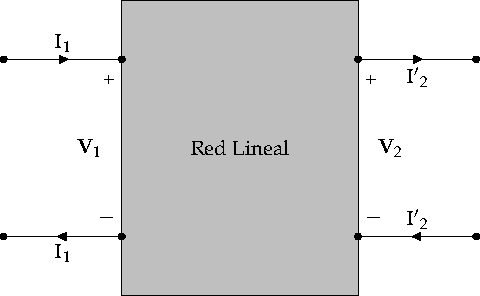
\includegraphics[width=.9\linewidth]{../figs/cuadripolo_transmision.pdf}
\end{center}

\[
  \left[
    \begin{array}{c}
      \mathbf{V}_1\\
      \mathbf{I}_1
    \end{array}
  \right] =
  \left[
    \begin{array}{cc}
      \mathbf{A} & \mathbf{B}\\
      \mathbf{C} & \mathbf{D}
    \end{array}
  \right] \cdot
  \left[
    \begin{array}{c}
      \mathbf{V}_2\\
      \mathbf{I'}_2
    \end{array}
  \right]
\]
\end{frame}

\begin{frame}[label={sec:org0ed6466}]{Cálculo de parámetros}
Se debe medir el inverso de cada parámetro, dado que la magnitud a medir y la excitación pertenecen al mismo puerto.

\renewcommand{\arraystretch}{3}
\[
  \begin{array}{cc}
    \frac{1}{\mathbf{A}} = \left.\frac{\mathbf{V}_2}{\mathbf{V}_1}\right\rvert_{\mathbf{I}_2 = 0} &
    \frac{1}{\mathbf{B}} = \left.\frac{\mathbf{I'}_2}{\mathbf{V}_1}\right\rvert_{\mathbf{V}_2 = 0}\\
    \frac{1}{\mathbf{C}} = \left.\frac{\mathbf{V}_2}{\mathbf{I}_1}\right\rvert_{\mathbf{I}_2 = 0} &
    \frac{1}{\mathbf{D}} = \left.\frac{\mathbf{I'}_2}{\mathbf{I}_1}\right\rvert_{\mathbf{V}_2 = 0}\\
  \end{array}
\]

\begin{columns}
\begin{column}{0.5\columnwidth}
\begin{center}
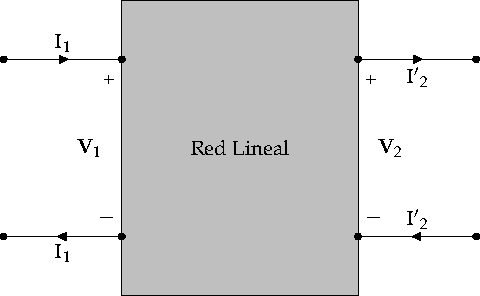
\includegraphics[width=.9\linewidth]{../figs/cuadripolo_transmision.pdf}
\end{center}
\end{column}

\begin{column}{0.5\columnwidth}
\renewcommand{\arraystretch}{1}
\[
\begin{array}{l}
  \mathbf{V}_1 = \mathbf{A} \mathbf{V}_2 + \mathbf{B}\mathbf{I'}_2\\
  \mathbf{I}_1 = \mathbf{C} \mathbf{V}_2 + \mathbf{D} \mathbf{I'}_2\\
\end{array}
\]
\end{column}
\end{columns}
\end{frame}


\subsection{Parámetros de Transmisión Inversa}
\label{sec:org1443865}

\begin{frame}[label={sec:orgb3ce5df}]{Definición}
\begin{center}
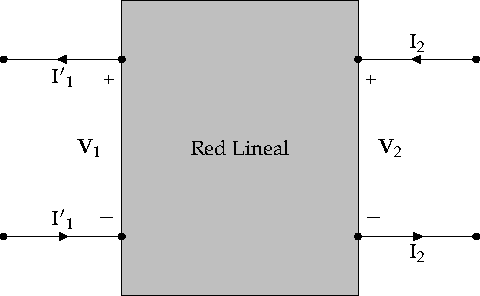
\includegraphics[width=.9\linewidth]{../figs/cuadripolo_transmision_inversa.pdf}
\end{center}

\[
\begin{array}{l}
  \mathbf{V}_2 = \mathbf{a} \mathbf{V}_1 + \mathbf{b}\mathbf{I'}_1\\
  \mathbf{I}_2 = \mathbf{c} \mathbf{V}_1 + \mathbf{d} \mathbf{I'}_1\\
\end{array}
\]

\begin{center}
\alert{Atención} al sentido de la corriente \(\mathbf{I'}_1\) (\(\mathbf{I'}_1 = - \mathbf{I}_1\)).
\end{center}
\end{frame}

\begin{frame}[label={sec:org855ab34}]{Expresión Matricial}
\begin{center}
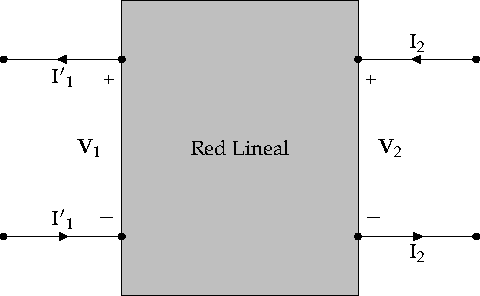
\includegraphics[width=.9\linewidth]{../figs/cuadripolo_transmision_inversa.pdf}
\end{center}

\[
  \left[
    \begin{array}{c}
      \mathbf{V}_2\\
      \mathbf{I}_2
    \end{array}
  \right] =
  \left[
    \begin{array}{cc}
      \mathbf{a} & \mathbf{b}\\
      \mathbf{c} & \mathbf{d}
    \end{array}
  \right] \cdot
  \left[
    \begin{array}{c}
      \mathbf{V}_1\\
      \mathbf{I'}_1
    \end{array}
  \right]
\]
\end{frame}

\begin{frame}[label={sec:org49369ab}]{Cálculo de parámetros}
Se debe medir el inverso de cada parámetro, dado que la magnitud a medir y la excitación pertenecen al mismo puerto.

\renewcommand{\arraystretch}{3}
\[
  \begin{array}{cc}
    \frac{1}{\mathbf{a}} = \left.\frac{\mathbf{V}_1}{\mathbf{V}_2}\right\rvert_{\mathbf{I}_1 = 0} &
    \frac{1}{\mathbf{b}} = \left.\frac{\mathbf{I'}_1}{\mathbf{V}_2}\right\rvert_{\mathbf{V}_1 = 0}\\
    \frac{1}{\mathbf{c}} = \left.\frac{\mathbf{V}_1}{\mathbf{I}_2}\right\rvert_{\mathbf{I}_1 = 0} &
    \frac{1}{\mathbf{d}} = \left.\frac{\mathbf{I'}_1}{\mathbf{I}_2}\right\rvert_{\mathbf{V}_1 = 0}\\
  \end{array}
\]

\begin{columns}
\begin{column}{0.5\columnwidth}
\begin{center}
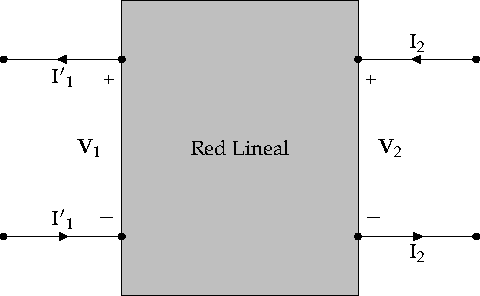
\includegraphics[width=.9\linewidth]{../figs/cuadripolo_transmision_inversa.pdf}
\end{center}
\end{column}

\begin{column}{0.5\columnwidth}
\renewcommand{\arraystretch}{1}
\[
\begin{array}{l}
  \mathbf{V}_2 = \mathbf{a} \mathbf{V}_1 + \mathbf{b}\mathbf{I'}_1\\
  \mathbf{I}_2 = \mathbf{c} \mathbf{V}_1 + \mathbf{d} \mathbf{I'}_1\\
\end{array}
\]
\end{column}
\end{columns}
\end{frame}


\section{Relación entre parámetros}
\label{sec:org28f423d}

\begin{frame}[label={sec:orgdd994e7}]{Impedancia y Admitancia}
\[
  \left.
    \begin{array}{l}
      \left[
      \begin{array}{c}
        \mathbf{V}_1\\
        \mathbf{V}_2
      \end{array}
      \right] =
      \left[
      \begin{array}{cc}
        \mathbf{z}_{11} & \mathbf{z}_{12}\\
        \mathbf{z}_{21} & \mathbf{z}_{22}
      \end{array}
                          \right]
                          \cdot
                          \left[
                          \begin{array}{c}
                            \mathbf{I}_1\\
                            \mathbf{I}_2
                          \end{array}
      \right] \\ \\
      \left[
      \begin{array}{c}
        \mathbf{I}_1\\
        \mathbf{I}_2
      \end{array}
      \right] =
      \left[
      \begin{array}{cc}
        \mathbf{y}_{11} & \mathbf{y}_{12}\\
        \mathbf{y}_{21} & \mathbf{y}_{22}
      \end{array}
                          \right] \cdot
                          \left[
                          \begin{array}{c}
                            \mathbf{V}_1\\
                            \mathbf{V}_2
                          \end{array}
      \right]
    \end{array}
    \right\}
      \rightarrow
      \boxed{[\mathbf{Z}] = [\mathbf{Y}]^{-1}}
    \]
\end{frame}

\begin{frame}[label={sec:orgcc3ffb4}]{Híbridos}
\[
  \left.
    \begin{array}{l}
      %% Híbridos
  \left[
    \begin{array}{c}
      \mathbf{V}_1\\
      \mathbf{I}_2
    \end{array}
  \right] =
  \left[
    \begin{array}{cc}
      \mathbf{h}_{11} & \mathbf{h}_{12}\\
      \mathbf{h}_{21} & \mathbf{h}_{22}
    \end{array}
  \right] \cdot
  \left[
    \begin{array}{c}
      \mathbf{I}_1\\
      \mathbf{V}_2
    \end{array}
      \right]
      \\ \\
      %% Híbridos Inversos
  \left[
    \begin{array}{c}
      \mathbf{I}_1\\
      \mathbf{V}_2
    \end{array}
  \right] =
  \left[
    \begin{array}{cc}
      \mathbf{g}_{11} & \mathbf{g}_{12}\\
      \mathbf{g}_{21} & \mathbf{g}_{22}
    \end{array}
  \right] \cdot
  \left[
    \begin{array}{c}
      \mathbf{V}_1\\
      \mathbf{I}_2
    \end{array}
      \right]
      \end{array}
    \right\}
      \rightarrow
      \boxed{[\mathbf{H}] = [\mathbf{G}]^{-1}}
    \]
\end{frame}
\begin{frame}[label={sec:org3938d90}]{Transmisión}
\[
  \left.
    \begin{array}{l}
      %% Transmisión
  \left[
    \begin{array}{c}
      \mathbf{V}_1\\
      \mathbf{I}_1
    \end{array}
  \right] =
  \left[
    \begin{array}{cc}
      \mathbf{A} & \mathbf{B}\\
      \mathbf{C} & \mathbf{D}
    \end{array}
  \right] \cdot
  \left[
    \begin{array}{c}
      \mathbf{V}_2\\
      \mathbf{I'}_2
    \end{array}
  \right]
      \\ \\
      %% Transmisión Inversa
  \left[
    \begin{array}{c}
      \mathbf{V}_2\\
      \mathbf{I}_2
    \end{array}
  \right] =
  \left[
    \begin{array}{cc}
      \mathbf{a} & \mathbf{b}\\
      \mathbf{c} & \mathbf{d}
    \end{array}
  \right] \cdot
  \left[
    \begin{array}{c}
      \mathbf{V}_1\\
      \mathbf{I'}_1
    \end{array}
  \right]
      \end{array}
    \right\}
    \rightarrow
    \boxed{[\mathbf{T}] \neq [\mathbf{t}]^{-1}}
  \]
\[
  \boxed{
    \left[
      \begin{array}{cc}
        \mathbf{A} & \mathbf{B}\\
        \mathbf{C} & \mathbf{D}
      \end{array}\right] = 
      \left[
      \begin{array}{cc}
        \mathbf{a} & \mathbf{-b}\\
        \mathbf{-c} & \mathbf{d}
      \end{array}
      \right]^{-1}
    }
\]
\end{frame}
\begin{frame}[label={sec:orgbc57381},plain]{}
\begin{center}
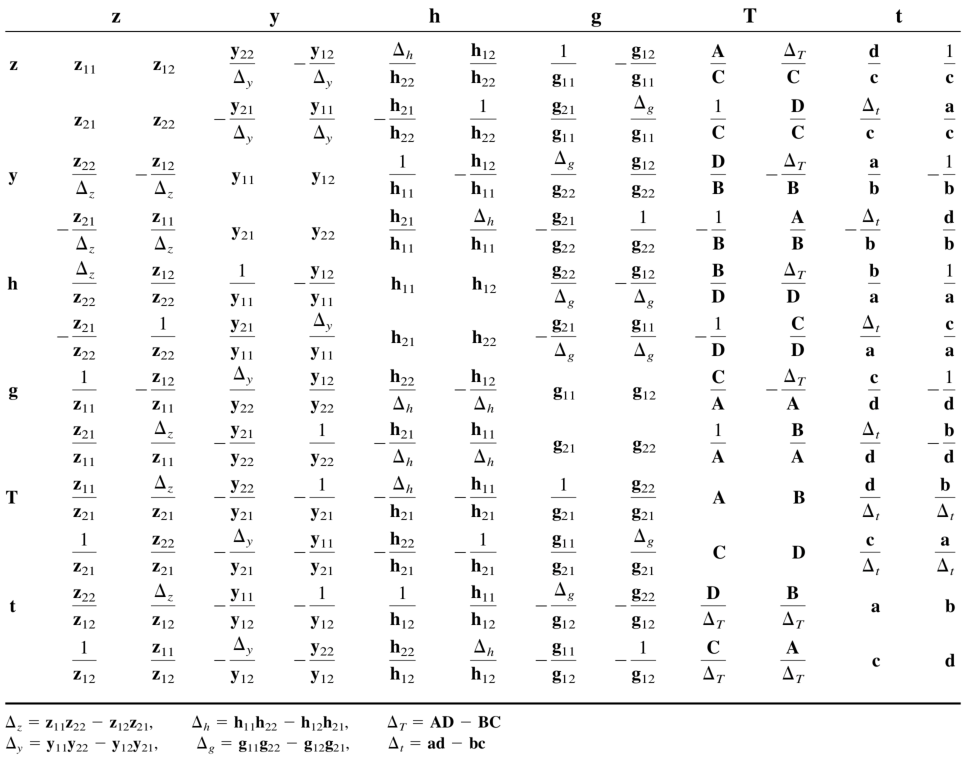
\includegraphics[width=1.15\textwidth]{../figs/Tabla_Parametros.pdf}
\end{center}
\end{frame}

\begin{frame}[label={sec:org65e1ba5}]{Reciprocidad}
A partir de las relaciones ya obtenidas para impedancia y admitancia, utilizando la tabla anterior obtenemos la relación para parámetros híbridos y de transmisión:
\[
\left.
\begin{array}{l}
  \mathbf{z_{12}} = \mathbf{z_{21}}\\
  \mathbf{y_{12}} = \mathbf{y_{21}}\\
\end{array}
\right\} \rightarrow
\left\{
\begin{array}{l}
  \mathbf{h_{12}} = - \mathbf{h_{21}}\\
  \mathbf{g_{12}} = - \mathbf{g_{21}}\\
  \mathbf{A} \mathbf{D} - \mathbf{B} \mathbf{C} = 1\\
  \mathbf{a} \mathbf{d} - \mathbf{b} \mathbf{c} = 1\\
\end{array}
\right.
\]
\end{frame}


\begin{frame}[label={sec:org13d9afa}]{Simetría}
A partir de las relaciones ya obtenidas para impedancia y admitancia, utilizando la tabla anterior obtenemos la relación para parámetros híbridos y de transmisión:
\[
\left.
\begin{array}{l}
  \mathbf{z_{11}} = \mathbf{z_{22}}\\
  \mathbf{y_{11}} = \mathbf{y_{22}}\\
\end{array}
\right\} \rightarrow
\left\{
\begin{array}{l}
  \mathbf{h_{11}} \cdot \mathbf{h_{22}} - \mathbf{h_{12}}^2 = 1\\
  \mathbf{g_{11}} \cdot \mathbf{g_{22}} - \mathbf{g_{12}}^2 = 1\\
  \mathbf{A} =  \mathbf{D}\\
  \mathbf{a} =  \mathbf{d}\\
\end{array}
\right.
\]

Además:

\[
  \boxed{[\mathbf{T}] = [\mathbf{t}]}
\]
\end{frame}


\section{Cuadripolos entre Dipolos Terminales}
\label{sec:org123cceb}

\subsection{Situación General}
\label{sec:orgaab4587}
\begin{frame}[label={sec:org4e2a4f5}]{}
\begin{center}
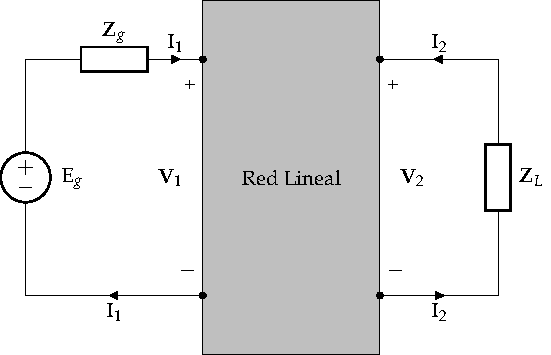
\includegraphics[width=.9\linewidth]{../figs/cuadripolo_cargado_fuente_tension.pdf}
\end{center}

\begin{align*}
  \mathbf{V}_1 &= \mathbf{E}_g - \mathbf{Z}_g \cdot \mathbf{I}_1\\
  \mathbf{V}_2 &= - \mathbf{Z}_L \cdot \mathbf{I}_2\\
\end{align*}
\end{frame}

\begin{frame}[label={sec:orgb4461a1}]{}
\begin{center}
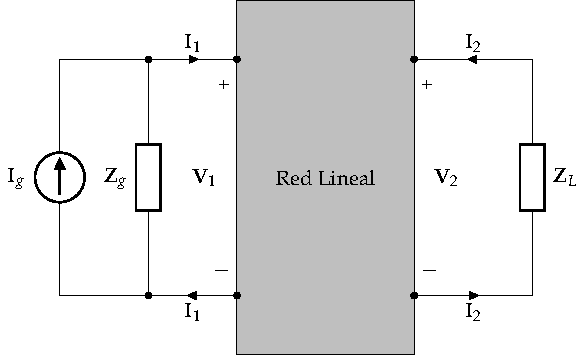
\includegraphics[width=.9\linewidth]{../figs/cuadripolo_cargado_fuente_corriente.pdf}
\end{center}

\begin{align*}
  \mathbf{V}_1 &= (\mathbf{I}_g - \mathbf{I}_1) \cdot \mathbf{Z}_g\\
  \mathbf{V}_2 &= - \mathbf{Z}_L \cdot \mathbf{I}_2\\
\end{align*}
\end{frame}

\begin{frame}[label={sec:org50c18ba}]{Ganancia}
\begin{columns}
\begin{column}{0.5\columnwidth}
\begin{center}
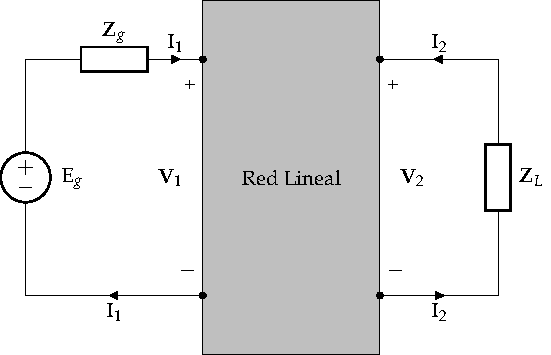
\includegraphics[width=.9\linewidth]{../figs/cuadripolo_cargado_fuente_tension.pdf}
\end{center}

\begin{center}
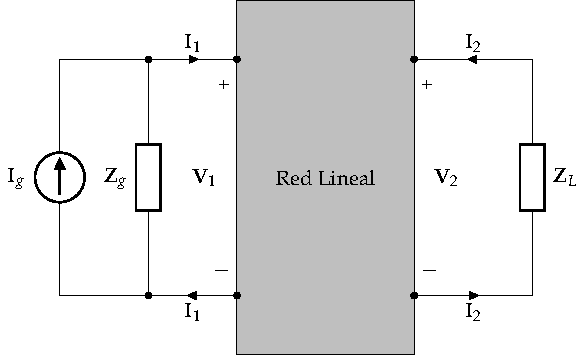
\includegraphics[width=.9\linewidth]{../figs/cuadripolo_cargado_fuente_corriente.pdf}
\end{center}
\end{column}


\begin{column}{0.5\columnwidth}
\begin{itemize}
\item Ganancia de Tensión
\end{itemize}
\[
\mathbf{A}_V = \frac{\mathbf{V}_2}{\mathbf{E}_g}
\]
\begin{itemize}
\item Ganancia de Corriente
\end{itemize}
\[
\mathbf{A}_I = \frac{\mathbf{I}_2}{\mathbf{I}_g}
\]
\end{column}
\end{columns}
\end{frame}

\begin{frame}[label={sec:orgeb0de1f}]{Impedancia}
\begin{columns}
\begin{column}{0.5\columnwidth}
\begin{center}
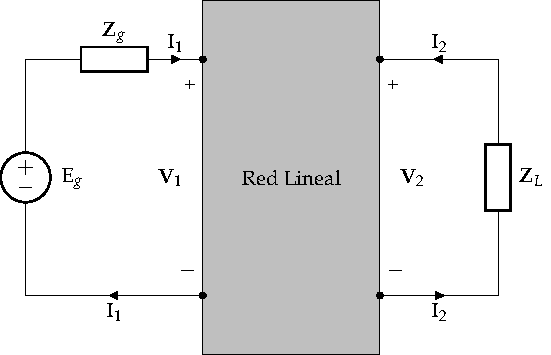
\includegraphics[width=.9\linewidth]{../figs/cuadripolo_cargado_fuente_tension.pdf}
\end{center}

\begin{center}
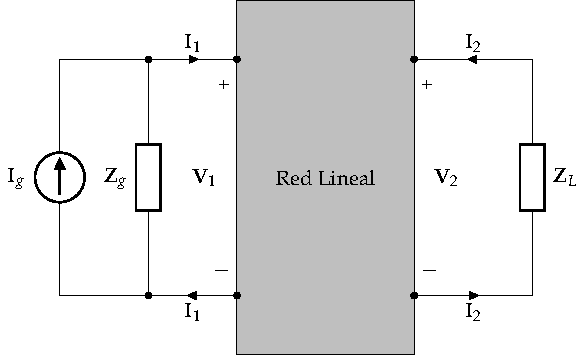
\includegraphics[width=.9\linewidth]{../figs/cuadripolo_cargado_fuente_corriente.pdf}
\end{center}
\end{column}


\begin{column}{0.5\columnwidth}
\begin{itemize}
\item Impedancia de Entrada
\end{itemize}
\[
\mathbf{Z}_i = \frac{\mathbf{V}_1}{\mathbf{I}_1}
\]

\begin{itemize}
\item Impedancia de Salida
\end{itemize}
\[
\mathbf{Z}_o = \left.\frac{\mathbf{V}_2}{\mathbf{I}_2}\right\rvert_{\mathbf{E}_g = 0}
\]
\end{column}
\end{columns}
\end{frame}

\begin{frame}[label={sec:org645bc44}]{Transferencia}
\begin{columns}
\begin{column}{0.5\columnwidth}
\begin{center}
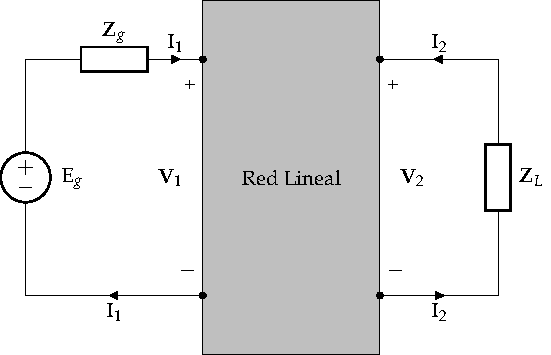
\includegraphics[width=.9\linewidth]{../figs/cuadripolo_cargado_fuente_tension.pdf}
\end{center}

\begin{center}
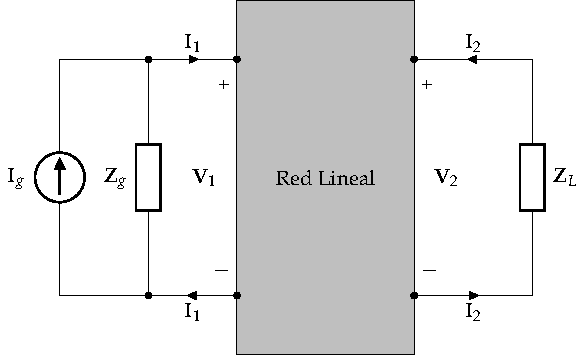
\includegraphics[width=.9\linewidth]{../figs/cuadripolo_cargado_fuente_corriente.pdf}
\end{center}
\end{column}


\begin{column}{0.5\columnwidth}
\begin{itemize}
\item Transadmitancia directa
\end{itemize}
\[
\mathbf{Y}_f = \frac{\mathbf{I}_2}{\mathbf{E}_g}
\]

\begin{itemize}
\item Transimpedancia directa
\end{itemize}
\[
\mathbf{Z}_f = \frac{\mathbf{V}_2}{\mathbf{I}_g}
\]
\end{column}
\end{columns}
\end{frame}

\begin{frame}[label={sec:orgeade01e}]{Ejercicio de Cálculo (1)}
Demuestra que la impedancia de entrada del circuito a la derecha de la fuente real expresada con parámetros de transmisión es:

\[
\mathbf{Z}_i = \frac{\mathbf{A} \mathbf{Z}_L + \mathbf{B}}{\mathbf{C}\mathbf{Z}_L + \mathbf{D}}
\]

\begin{center}
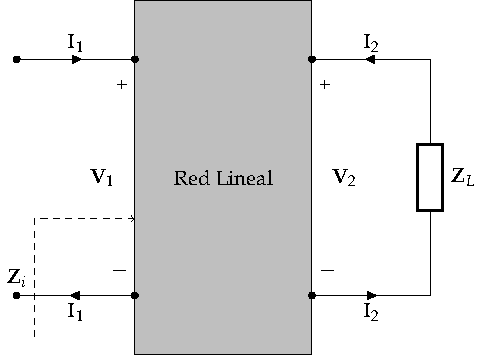
\includegraphics[height=0.6\textheight]{../figs/cuadripolo_cargado_impedancia_entrada.pdf}
\end{center}
\end{frame}



\begin{frame}[label={sec:org9388793}]{Ejercicio de Cálculo (2)}
¿Qué impedancia de carga \(\mathbf{Z}_L\) hay que conectar a la salida del cuadripolo para obtener la máxima transferencia de potencia?


\begin{center}
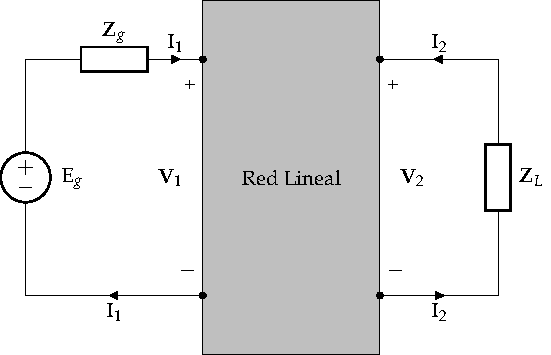
\includegraphics[width=.9\linewidth]{../figs/cuadripolo_cargado_fuente_tension.pdf}
\end{center}
\end{frame}

\subsection{Parámetros Imagen}
\label{sec:org5f4e5de}

\begin{frame}[label={sec:org49d5911}]{Impedancia Característica}
Para un cuadripolo \alert{recíproco} y \alert{simétrico} se definen los parámetros imagen:

\begin{itemize}
\item \alert{Impedancia característica}, \(\mathbf{Z}_o\): impedancia que, conectada en una puerta, hace que desde la otra puerta se vea la misma impedancia.
\end{itemize}
\[
  \mathbf{Z}_o = \frac{\mathbf{U}_1}{\mathbf{I}_1}
\]

\begin{columns}
\begin{column}{0.7\columnwidth}
\begin{center}
\includegraphics[width=.9\linewidth]{../figs/cuadripolo_impedancia_caracteristica.pdf}
\end{center}
\end{column}

\begin{column}{0.4\columnwidth}
\[
\mathbf{Z}_o = \frac{\mathbf{A} \mathbf{Z}_o + \mathbf{B}}{\mathbf{C}\mathbf{Z}_o + \mathbf{D}}
\]

\[
\mathbf{A} = \mathbf{D} \rightarrow \boxed{\mathbf{Z}_o = \pm \sqrt{\frac{\mathbf{B}}{\mathbf{C}}}}
\]
\end{column}
\end{columns}
\end{frame}

\begin{frame}[label={sec:orge0f8e2f}]{Impedancia Característica}
\begin{block}{Atención}
La ecuación proporciona dos soluciones, una de las cuáles implicará una impedancia no viable (\emph{resistencia negativa}).
\[
\boxed{\mathbf{Z}_o = \pm \sqrt{\frac{\mathbf{B}}{\mathbf{C}}}}
\]
\end{block}
\end{frame}

\begin{frame}[label={sec:orgc027250}]{Función de Propagación}
Para un cuadripolo \alert{recíproco} y \alert{simétrico} se definen los parámetros imagen:

\begin{itemize}
\item \alert{Función de propagación}, \(\gamma\): relacionada con el cociente de potencias en las puertas del cuadripolo cuando una de ellas está cargada con \(\mathbf{Z}_o\)
\end{itemize}

\[
  \exp(2\gamma) = \frac{\mathbf{U}_1\mathbf{I}_1}{\mathbf{U}_2\mathbf{I}'_2}
\]

\begin{columns}
\begin{column}{0.6\columnwidth}
\begin{center}
\includegraphics[width=.9\linewidth]{../figs/cuadripolo_impedancia_caracteristica.pdf}
\end{center}
\end{column}

\begin{column}{0.4\columnwidth}
\begin{align*}
  \mathbf{U}_1 &= \mathbf{I}_1 \mathbf{Z}_o\\
  \mathbf{U}_2 &= \mathbf{I}'_2 \mathbf{Z}_o
\end{align*}

\[
  \boxed{\exp(\gamma) = \frac{\mathbf{U}_1}{\mathbf{U}_2} = \frac{\mathbf{I}_1}{\mathbf{I}'_2}}
\]
\end{column}
\end{columns}
\end{frame}


\begin{frame}[label={sec:orgd96bd25}]{Relación entre \(\mathbf{Z}_o\) y \(\gamma\)}
\begin{columns}
\begin{column}{0.6\columnwidth}
\begin{center}
\includegraphics[width=.9\linewidth]{../figs/cuadripolo_impedancia_caracteristica.pdf}
\end{center}
\end{column}

\begin{column}{0.4\columnwidth}
\begin{align*}
  \exp(\gamma) &= \frac{\mathbf{U}_1}{\mathbf{U}_2} =\\
               &= \frac{\mathbf{A}\mathbf{U}_2 + \mathbf{B}\mathbf{I}'_2}{\mathbf{U}_2} = \\
               &= \mathbf{A} + \mathbf{B}\frac{\mathbf{I}'_2}{\mathbf{U_2}}
\end{align*}

\[
  \boxed{\exp(\gamma) = \mathbf{A} + \frac{\mathbf{B}}{\mathbf{Z}_o}}
\]
\end{column}
\end{columns}
\end{frame}

\begin{frame}[label={sec:orgdca4369}]{Relación entre \(\mathbf{Z}_o\) y \(\gamma\)}
Teniendo en cuenta la expresión de \(\mathbf{Z}_o\):
\[
  \left.
  \begin{array}{l}
    \mathbf{Z}_o = \pm \sqrt{\frac{\mathbf{B}}{\mathbf{C}}}\\
    \exp(\gamma) = \mathbf{A} + \frac{\mathbf{B}}{\mathbf{Z}_o}
  \end{array} \right\} \rightarrow
\boxed{\exp(\gamma) = \mathbf{A} \pm \sqrt{\mathbf{B}\mathbf{C}}}
\]

Además, teniendo en cuenta la relación de un cuadripolo recíproco y simétrico:

\[
  \mathbf{A}^2 - \mathbf{B}\mathbf{C} = 1 \rightarrow %
  \boxed{\exp(\gamma) = \mathbf{A} \pm \sqrt{\mathbf{A}^2 - 1}}
\]
\alert{Atención} al signo que acompaña a las raíces cuadradas. Se debe elegir de forma que la parte real de \(\gamma\) sea acorde al cuadripolo.
\end{frame}

\begin{frame}[label={sec:org961e306}]{Transmisión a partir de Imagen}
\[
\mathbf{A}^2 - \mathbf{B}\mathbf{C} = 1
\]

\begin{columns}
\begin{column}{0.33\columnwidth}
\[
  e^\gamma = \mathbf{A} + \sqrt{\mathbf{A}^2 - 1}
\]

\[
  \mathbf{Z}_o = \sqrt{\frac{\mathbf{B}}{\mathbf{C}}}
\]
\end{column}

\begin{column}{0.33\columnwidth}
\begin{align*}
  \cosh(\gamma) &= \frac{e^\gamma + e^{-\gamma}}{2}\\
  \sinh(\gamma) &= \frac{e^\gamma - e^{-\gamma}}{2}\\
  \cosh^2(\gamma) &- \sinh^2(\gamma) = 1
\end{align*}
\end{column}
\end{columns}

\vspace{1cm}
\[
\boxed{
  \begin{array}{ll}
    \mathbf{A} = \cosh(\gamma) &
    \mathbf{B} = \mathbf{Z}_o \sinh(\gamma)\\
    \mathbf{C} = \sinh(\gamma)/\mathbf{Z}_o &
    \mathbf{D} = \cosh(\gamma)\\
  \end{array}
}
\]
\end{frame}

\begin{frame}[label={sec:org43b8179}]{Régimen Permanente Sinusoidal}
Cuando el circuito funciona en régimen permanente sinusoidal:

\begin{itemize}
\item La función de propagación es un número complejo denominado constante de propagación.
\end{itemize}
\[
  \overline{\gamma} = \alpha + j\beta
\]
\begin{itemize}
\item Las tensiones y corrientes son fasores
\end{itemize}
\[
  \exp(\overline{\gamma}) = \exp(\alpha) \cdot \exp(j\beta) = \frac{\overline{U}_1}{\overline{U}_2} = \frac{\overline{I}_1}{\overline{I}'_2}
\]
\end{frame}

\begin{frame}[label={sec:orgda6f4f9}]{Régimen Permanente Sinusoidal}
\begin{itemize}
\item \alert{Constante de Atenuación} (cuando \(\alpha > 1\) el cuadripolo atenúa la salida respecto de la entrada)
\end{itemize}
\[
  \exp(\alpha) = \frac{U_1}{U_2} = \frac{I_1}{I_2}
\]
\begin{itemize}
\item \alert{Constante de Fase} (desfase entre puertos)
\end{itemize}
\[
  \beta = \theta_{\overline{U}_1} - \theta_{\overline{U}_2} = \theta_{\overline{I}_1} - \theta_{\overline{I}'_2}
\]
\end{frame}

\begin{frame}[label={sec:org4756e00}]{Atenuación de Potencia}
\alert{Cuando está conectada la impedancia característica}, las potencias activas en los puertos se expresan:

\begin{align*}
  P_1 &= U_1 I_1 \cos(\theta_o)\\
  P_2 &= U_2 I_2 \cos(\theta_o)
\end{align*}
donde \(\theta_o\) es el ángulo de la impedancia \(\overline{Z}_o\).

Por tanto, la relación de potencias activas es:

\[
\frac{P_1}{P_2} = \frac{U_1 I_1}{U_2 I_2}
\]
Teniendo en cuenta la expresión de la constante de atenuación, esta relación es:
\[
    \exp(\alpha) = \frac{U_1}{U_2} = \frac{I_1}{I_2} \rightarrow \boxed{\exp(2\alpha) = \frac{U_1 I_1}{U_2 I_1} = \frac{P_1}{P_2}}
\]
\end{frame}

\section{Asociación de Cuadripolos}
\label{sec:org54130c5}

\begin{frame}[label={sec:org7c0040c}]{Conexiones}
\begin{block}{Definición}
\begin{itemize}
\item \alert{Serie}: misma corriente, suma de tensiones
\item \alert{Paralelo}: misma tensión, suma de corrientes
\end{itemize}
\end{block}
\begin{block}{Catálogo}
\begin{itemize}
\item Serie-Serie: \alert{parámetros impedancia}
\item Paralelo-Paralelo: \alert{parámetros admitancia}
\item Serie-Paralelo: \alert{parámetros híbridos}
\item Paralelo-Serie: \alert{parámetros híbridos inversos}
\item Cascada: \alert{parámetros transmisión/imagen}
\end{itemize}
\end{block}
\end{frame}
\subsection{Asociación Serie-Serie}
\label{sec:org8e78d0c}

\begin{frame}[label={sec:orgf80f396}]{Conexión}
\begin{columns}
\begin{column}{0.7\columnwidth}
\begin{center}
\includegraphics[height=0.85\textheight]{../figs/serie-serie.pdf}
\end{center}
\end{column}



\begin{column}{0.3\columnwidth}
\begin{block}{Tensiones}
\begin{align*}
  \mathbf{V}_1 &= \mathbf{V}_{1A} + \mathbf{V}_{1B}\\
  \mathbf{V}_2 &= \mathbf{V}_{2A} + \mathbf{V}_{2B}
\end{align*}
\end{block}

\begin{block}{Condición de Puerto}
\begin{align*}
  \mathbf{I}_{1A} &= \mathbf{I}_{1'A}\\
  \mathbf{I}_{1B} &= \mathbf{I}_{1'B}\\
  \mathbf{I}_{2A} &= \mathbf{I}_{2'A}\\
  \mathbf{I}_{2B} &= \mathbf{I}_{2'B}
\end{align*}
\end{block}
\end{column}
\end{columns}
\end{frame}

\begin{frame}[label={sec:org7523d8d}]{Cuadripolo Equivalente}
\begin{columns}
\begin{column}{0.65\columnwidth}
\begin{center}
\includegraphics[height=0.85\textheight]{../figs/serie-serie.pdf}
\end{center}
\end{column}


\begin{column}{0.35\columnwidth}
\begin{block}{Parámetros Impedancia}
\begin{align*}
  [\mathbf{V}_A] &= [\mathbf{Z}_A] \cdot [\mathbf{I}_A]\\
  [\mathbf{V}_B] &= [\mathbf{Z}_B] \cdot [\mathbf{I}_B]
\end{align*}
\end{block}

\begin{block}{Cuadripolo Equivalente}
\[
  \boxed{[\mathbf{Z}] = [\mathbf{Z}_A] + [\mathbf{Z}_B]}
\]
\end{block}
\end{column}
\end{columns}
\end{frame}

\begin{frame}[label={sec:orgbea9c05},plain]{Interacción}
\begin{columns}
\begin{column}{0.9\columnwidth}
\begin{center}
\includegraphics[width=.9\linewidth]{../figs/serie-serie-interaccion.pdf}
\end{center}
\end{column}
\begin{column}{0.3\columnwidth}
\begin{itemize}
\item Entrada
\end{itemize}
\begin{align*}
  \mathbf{I}_{1A} &= \mathbf{I}_{g1}\\
  \mathbf{I}_{1'A} &= \mathbf{I}_{g1} - \mathbf{I}_h
\end{align*}
\begin{itemize}
\item Salida
\end{itemize}
\begin{align*}
  \mathbf{I}_{2A} &= \mathbf{I}_{g2}\\
  \mathbf{I}_{2'A} &= \mathbf{I}_{g2}  + \mathbf{I}_h
\end{align*}
\begin{itemize}
\item Condición de Puerto
\end{itemize}
\[
\boxed{\mathbf{I}_h = 0}
\]
\end{column}
\end{columns}
\end{frame}
\begin{frame}[label={sec:org0818282},plain]{Interacción}
Si no hay interacción, al aplicar superposición la corriente de circulación debe ser nula \alert{en ambos casos}.
\begin{columns}
\begin{column}{0.65\columnwidth}
\begin{center}
\includegraphics[width=.9\linewidth]{../figs/serie-serie-superposicion-entrada.pdf}
\end{center}
\end{column}
\begin{column}{0.65\columnwidth}
\begin{center}
\includegraphics[width=.9\linewidth]{../figs/serie-serie-superposicion-salida.pdf}
\end{center}
\end{column}
\end{columns}
\end{frame}

\begin{frame}[label={sec:orgabb371a},plain]{Test de Brune}
Aplicando superposición desconectamos los cuadripolos: \alert{si no hay interacción, no habrá cambio de tensión}.
\begin{columns}
\begin{column}{0.65\columnwidth}
\begin{center}
\includegraphics[width=.9\linewidth]{../figs/serie-serie-brune-entrada.pdf}
\end{center}
\end{column}
\begin{column}{0.65\columnwidth}
\begin{center}
\includegraphics[width=.9\linewidth]{../figs/serie-serie-brune-salida.pdf}
\end{center}
\end{column}
\end{columns}
\end{frame}


\begin{frame}[label={sec:orge1383b0}]{Métodos para evitar interacción}
\begin{center}
\includegraphics[height=0.9\textheight]{../figs/serie-serie-transformador.pdf}
\end{center}
\end{frame}

\begin{frame}[label={sec:org76c1858}]{Métodos para evitar interacción}
\begin{center}
\includegraphics[height=0.9\textheight]{../figs/serie-serie-corto.pdf}
\end{center}
\end{frame}

\subsection{Asociación Paralelo-Paralelo}
\label{sec:org12174ff}
\begin{frame}[label={sec:orgd5cf4bc}]{Conexión}
\begin{columns}
\begin{column}{0.7\columnwidth}
\begin{center}
\includegraphics[height=0.75\textheight]{../figs/paralelo-paralelo.pdf}
\end{center}
\end{column}
\begin{column}{0.3\columnwidth}
\begin{block}{Corrientes}
\begin{align*}
  \mathbf{I}_1 &= \mathbf{I}_{1A} + \mathbf{I}_{1B}\\
  \mathbf{I}_2 &= \mathbf{I}_{2A} + \mathbf{I}_{2B}
\end{align*}
\end{block}

\begin{block}{Condición de Puerto}
\begin{align*}
  \mathbf{I}_{1A} &= \mathbf{I}_{1'A}\\
  \mathbf{I}_{1B} &= \mathbf{I}_{1'B}\\
  \mathbf{I}_{2A} &= \mathbf{I}_{2'A}\\
  \mathbf{I}_{2B} &= \mathbf{I}_{2'B}
\end{align*}
\end{block}
\end{column}
\end{columns}
\end{frame}

\begin{frame}[label={sec:orgdc513b5}]{Cuadripolo Equivalente}
\begin{columns}
\begin{column}{0.65\columnwidth}
\begin{center}
\includegraphics[height=0.7\textheight]{../figs/paralelo-paralelo.pdf}
\end{center}
\end{column}


\begin{column}{0.35\columnwidth}
\begin{block}{Parámetros Admitancia}
\begin{align*}
  [\mathbf{I}_A] &= [\mathbf{Y}_A] \cdot [\mathbf{V}_A]\\
  [\mathbf{I}_B] &= [\mathbf{Y}_B] \cdot [\mathbf{V}_B]
\end{align*}
\end{block}

\begin{block}{Cuadripolo Equivalente}
\[
  \boxed{[\mathbf{Y}] = [\mathbf{Y}_A] + [\mathbf{Y}_B]}
\]
\end{block}
\end{column}
\end{columns}
\end{frame}
\begin{frame}[label={sec:org8a3891f}]{Interacción}
\begin{center}
\includegraphics[height=0.9\textheight]{../figs/paralelo-paralelo-interaccion.pdf}
\end{center}
\end{frame}
\begin{frame}[label={sec:org12088a9},plain]{Interacción}
Si no hay interacción, al aplicar superposición la corriente de circulación debe ser nula \alert{en ambos casos}.
\begin{columns}
\begin{column}{0.65\columnwidth}
\begin{center}
\includegraphics[width=.9\linewidth]{../figs/paralelo-paralelo-superposicion-entrada.pdf}
\end{center}
\end{column}
\begin{column}{0.65\columnwidth}
\begin{center}
\includegraphics[width=.9\linewidth]{../figs/paralelo-paralelo-superposicion-salida.pdf}
\end{center}
\end{column}
\end{columns}
\end{frame}

\begin{frame}[label={sec:org5d7984d},plain]{Test de Brune}
Aplicando superposición desconectamos los cuadripolos: \alert{si no hay interacción, no habrá cambio de tensión}.
\begin{columns}
\begin{column}{0.65\columnwidth}
\begin{center}
\includegraphics[width=.9\linewidth]{../figs/paralelo-paralelo-brune-entrada.pdf}
\end{center}
\end{column}
\begin{column}{0.65\columnwidth}
\begin{center}
\includegraphics[width=.9\linewidth]{../figs/paralelo-paralelo-brune-salida.pdf}
\end{center}
\end{column}
\end{columns}
\end{frame}

\begin{frame}[label={sec:org54eecf6},plain]{Test de Brune}
Aplicando superposición desconectamos los cuadripolos: \alert{si no hay interacción, no habrá cambio de tensión}.
\begin{columns}
\begin{column}{0.65\columnwidth}
\begin{center}
\includegraphics[width=.9\linewidth]{../figs/paralelo-paralelo-brune-entrada2.pdf}
\end{center}
\end{column}
\begin{column}{0.65\columnwidth}
\begin{center}
\includegraphics[width=.9\linewidth]{../figs/paralelo-paralelo-brune-salida2.pdf}
\end{center}
\end{column}
\end{columns}
\end{frame}

\begin{frame}[label={sec:orgbf99fc5}]{Métodos para evitar interacción}
\begin{center}
\includegraphics[height=0.9\textheight]{../figs/paralelo-paralelo-transformador.pdf}
\end{center}
\end{frame}
\begin{frame}[label={sec:org9d5bb4e}]{Métodos para evitar interacción}
\begin{center}
\includegraphics[height=0.9\textheight]{../figs/paralelo-paralelo-corto.pdf}
\end{center}
\end{frame}
\subsection{Asociación Serie-Paralelo}
\label{sec:orgbd10eb0}
\begin{frame}[label={sec:orgde2eca9}]{Conexión}
\begin{columns}
\begin{column}{0.7\columnwidth}
\begin{center}
\includegraphics[height=0.75\textheight]{../figs/serie-paralelo.pdf}
\end{center}
\end{column}
\begin{column}{0.35\columnwidth}
\begin{block}{Relaciones}
\begin{align*}
  \mathbf{V}_1 &= \mathbf{V}_{1A} + \mathbf{V}_{1B}\\
  \mathbf{I}_2 &= \mathbf{I}_{2A} + \mathbf{I}_{2B}
\end{align*}
\end{block}

\begin{block}{Cuadripolo Equivalente}
\[
  \boxed{[\mathbf{H}] = [\mathbf{H}_A] + [\mathbf{H}_B]}
\]
\end{block}
\end{column}
\end{columns}
\end{frame}
\begin{frame}[label={sec:org0866253},plain]{Test de Brune}
Aplicando superposición desconectamos los cuadripolos: \alert{si no hay interacción, no habrá cambio de tensión}.
\begin{columns}
\begin{column}{0.65\columnwidth}
\begin{center}
\includegraphics[width=.9\linewidth]{../figs/serie-paralelo-brune-entrada.pdf}
\end{center}
\end{column}
\begin{column}{0.65\columnwidth}
\begin{center}
\includegraphics[width=.9\linewidth]{../figs/serie-paralelo-brune-salida.pdf}
\end{center}
\end{column}
\end{columns}
\end{frame}

\subsection{Asociación Paralelo-Serie}
\label{sec:org96cbb34}
\begin{frame}[label={sec:org9af3c80}]{Conexión}
\begin{columns}
\begin{column}{0.7\columnwidth}
\begin{center}
\includegraphics[height=0.75\textheight]{../figs/paralelo-serie.pdf}
\end{center}
\end{column}
\begin{column}{0.35\columnwidth}
\begin{block}{Relaciones}
\begin{align*}
  \mathbf{I}_1 &= \mathbf{I}_{1A} + \mathbf{I}_{1B}\\
  \mathbf{V}_2 &= \mathbf{V}_{2A} + \mathbf{V}_{2B}
\end{align*}
\end{block}

\begin{block}{Cuadripolo Equivalente}
\[
  \boxed{[\mathbf{G}] = [\mathbf{G}_A] + [\mathbf{G}_B]}
\]
\end{block}
\end{column}
\end{columns}
\end{frame}

\begin{frame}[label={sec:org75273b2},plain]{Test de Brune}
Aplicando superposición desconectamos los cuadripolos: \alert{si no hay interacción, no habrá cambio de tensión}.
\begin{columns}
\begin{column}{0.65\columnwidth}
\begin{center}
\includegraphics[width=.9\linewidth]{../figs/paralelo-serie-brune-entrada.pdf}
\end{center}
\end{column}
\begin{column}{0.65\columnwidth}
\begin{center}
\includegraphics[width=.9\linewidth]{../figs/paralelo-serie-brune-salida.pdf}
\end{center}
\end{column}
\end{columns}
\end{frame}
\subsection{Asociación Cascada}
\label{sec:orgf91c588}

\begin{frame}[label={sec:orgef71508}]{Conexión}
\begin{center}
\includegraphics[width=.9\linewidth]{../figs/cascada.pdf}
\end{center}

\begin{align*}
  \mathbf{V}_{2A} &= \mathbf{V}_{1B}\\
  \mathbf{I}'_{2A} &= \mathbf{I}_{1B}
\end{align*}


\[
  \boxed{[\mathbf{T}] = [\mathbf{T}_A] \cdot [\mathbf{T}_B]}
\]
\end{frame}
\end{document}